\subsection{High throughput binding affinity calculator}

(Stefan/Jumana)

HT BAC is a workflow system that uses RADICAL-Cybertools to implement ESMACS protocol, consisting of concurrent multi-stage consecutive MD runs followed by post processing steps. HT BAC uses the EnTK API to express this workflow, which provides the required high-throughput capabilities. 

\begin{figure}[tb]
\centering
  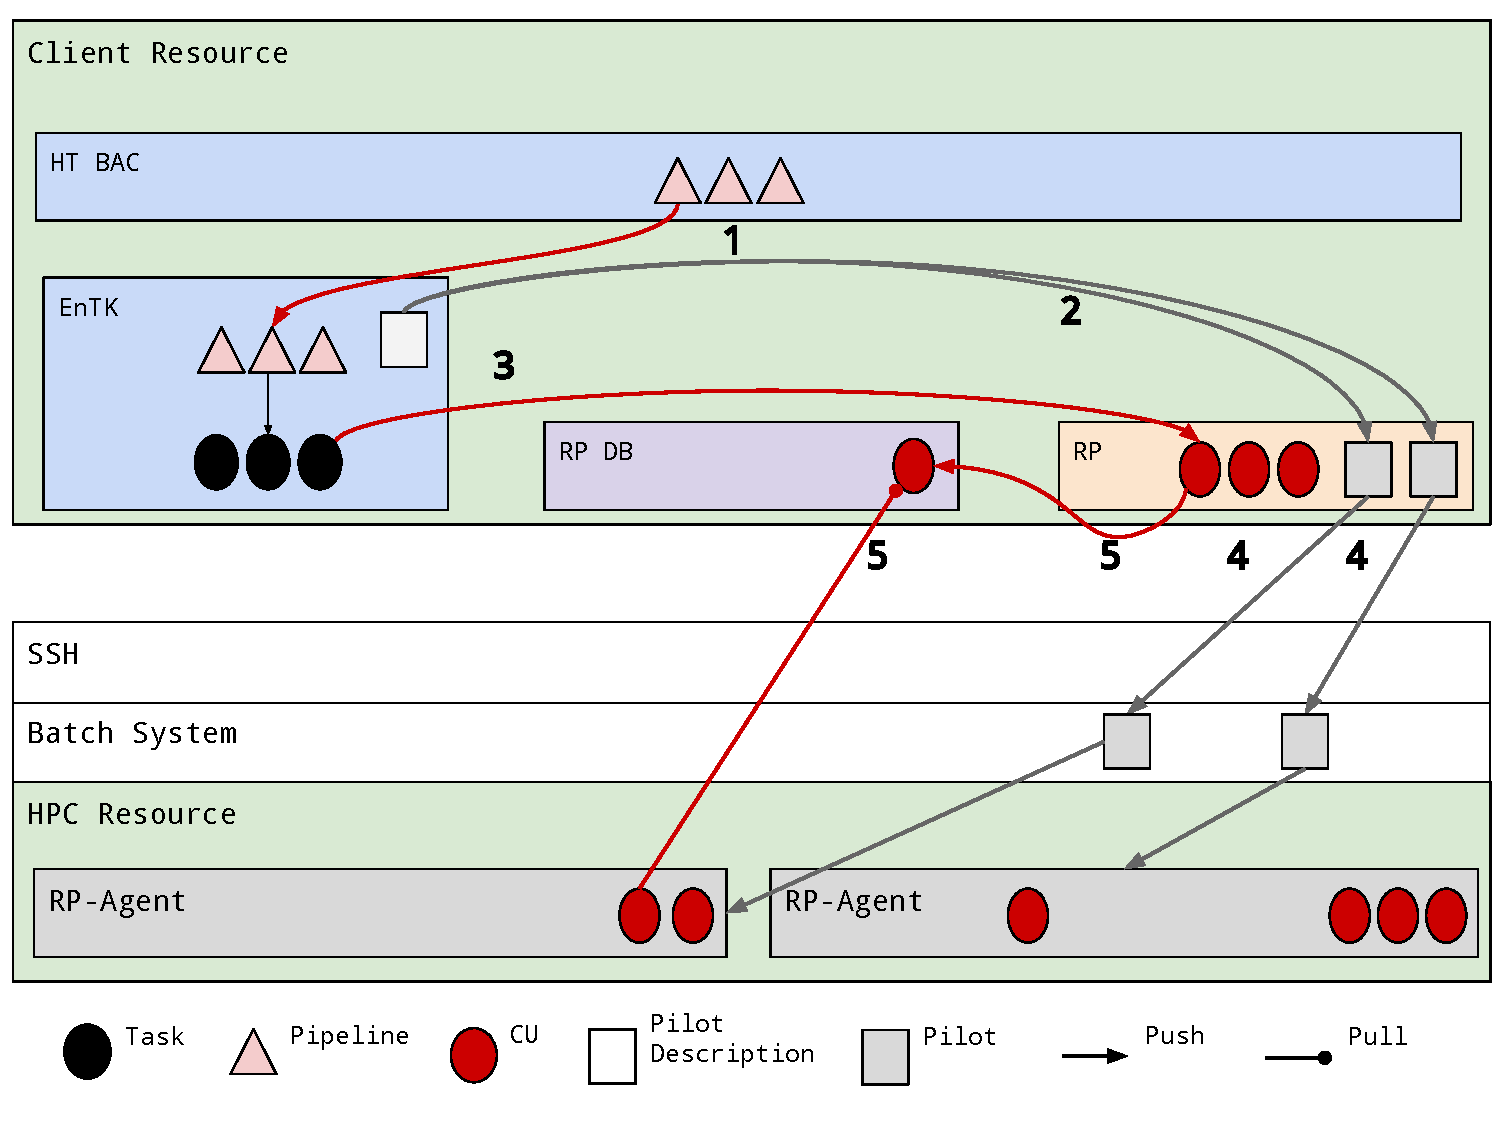
\includegraphics[width=0.4\textwidth]{FIGURES/ht-bac-rp_integration.pdf}
  \caption{\bf Integration between HT-BAC workflow system and EnTK. Numbers indicate the temporal sequence of execution. RADICAL-Pilot (RP) database (DB) can be deployed on any host reachable from the resources.}
   \label{figure:ht-bac_rp}
\end{figure}

\begin{figure}[tb]
\centering
  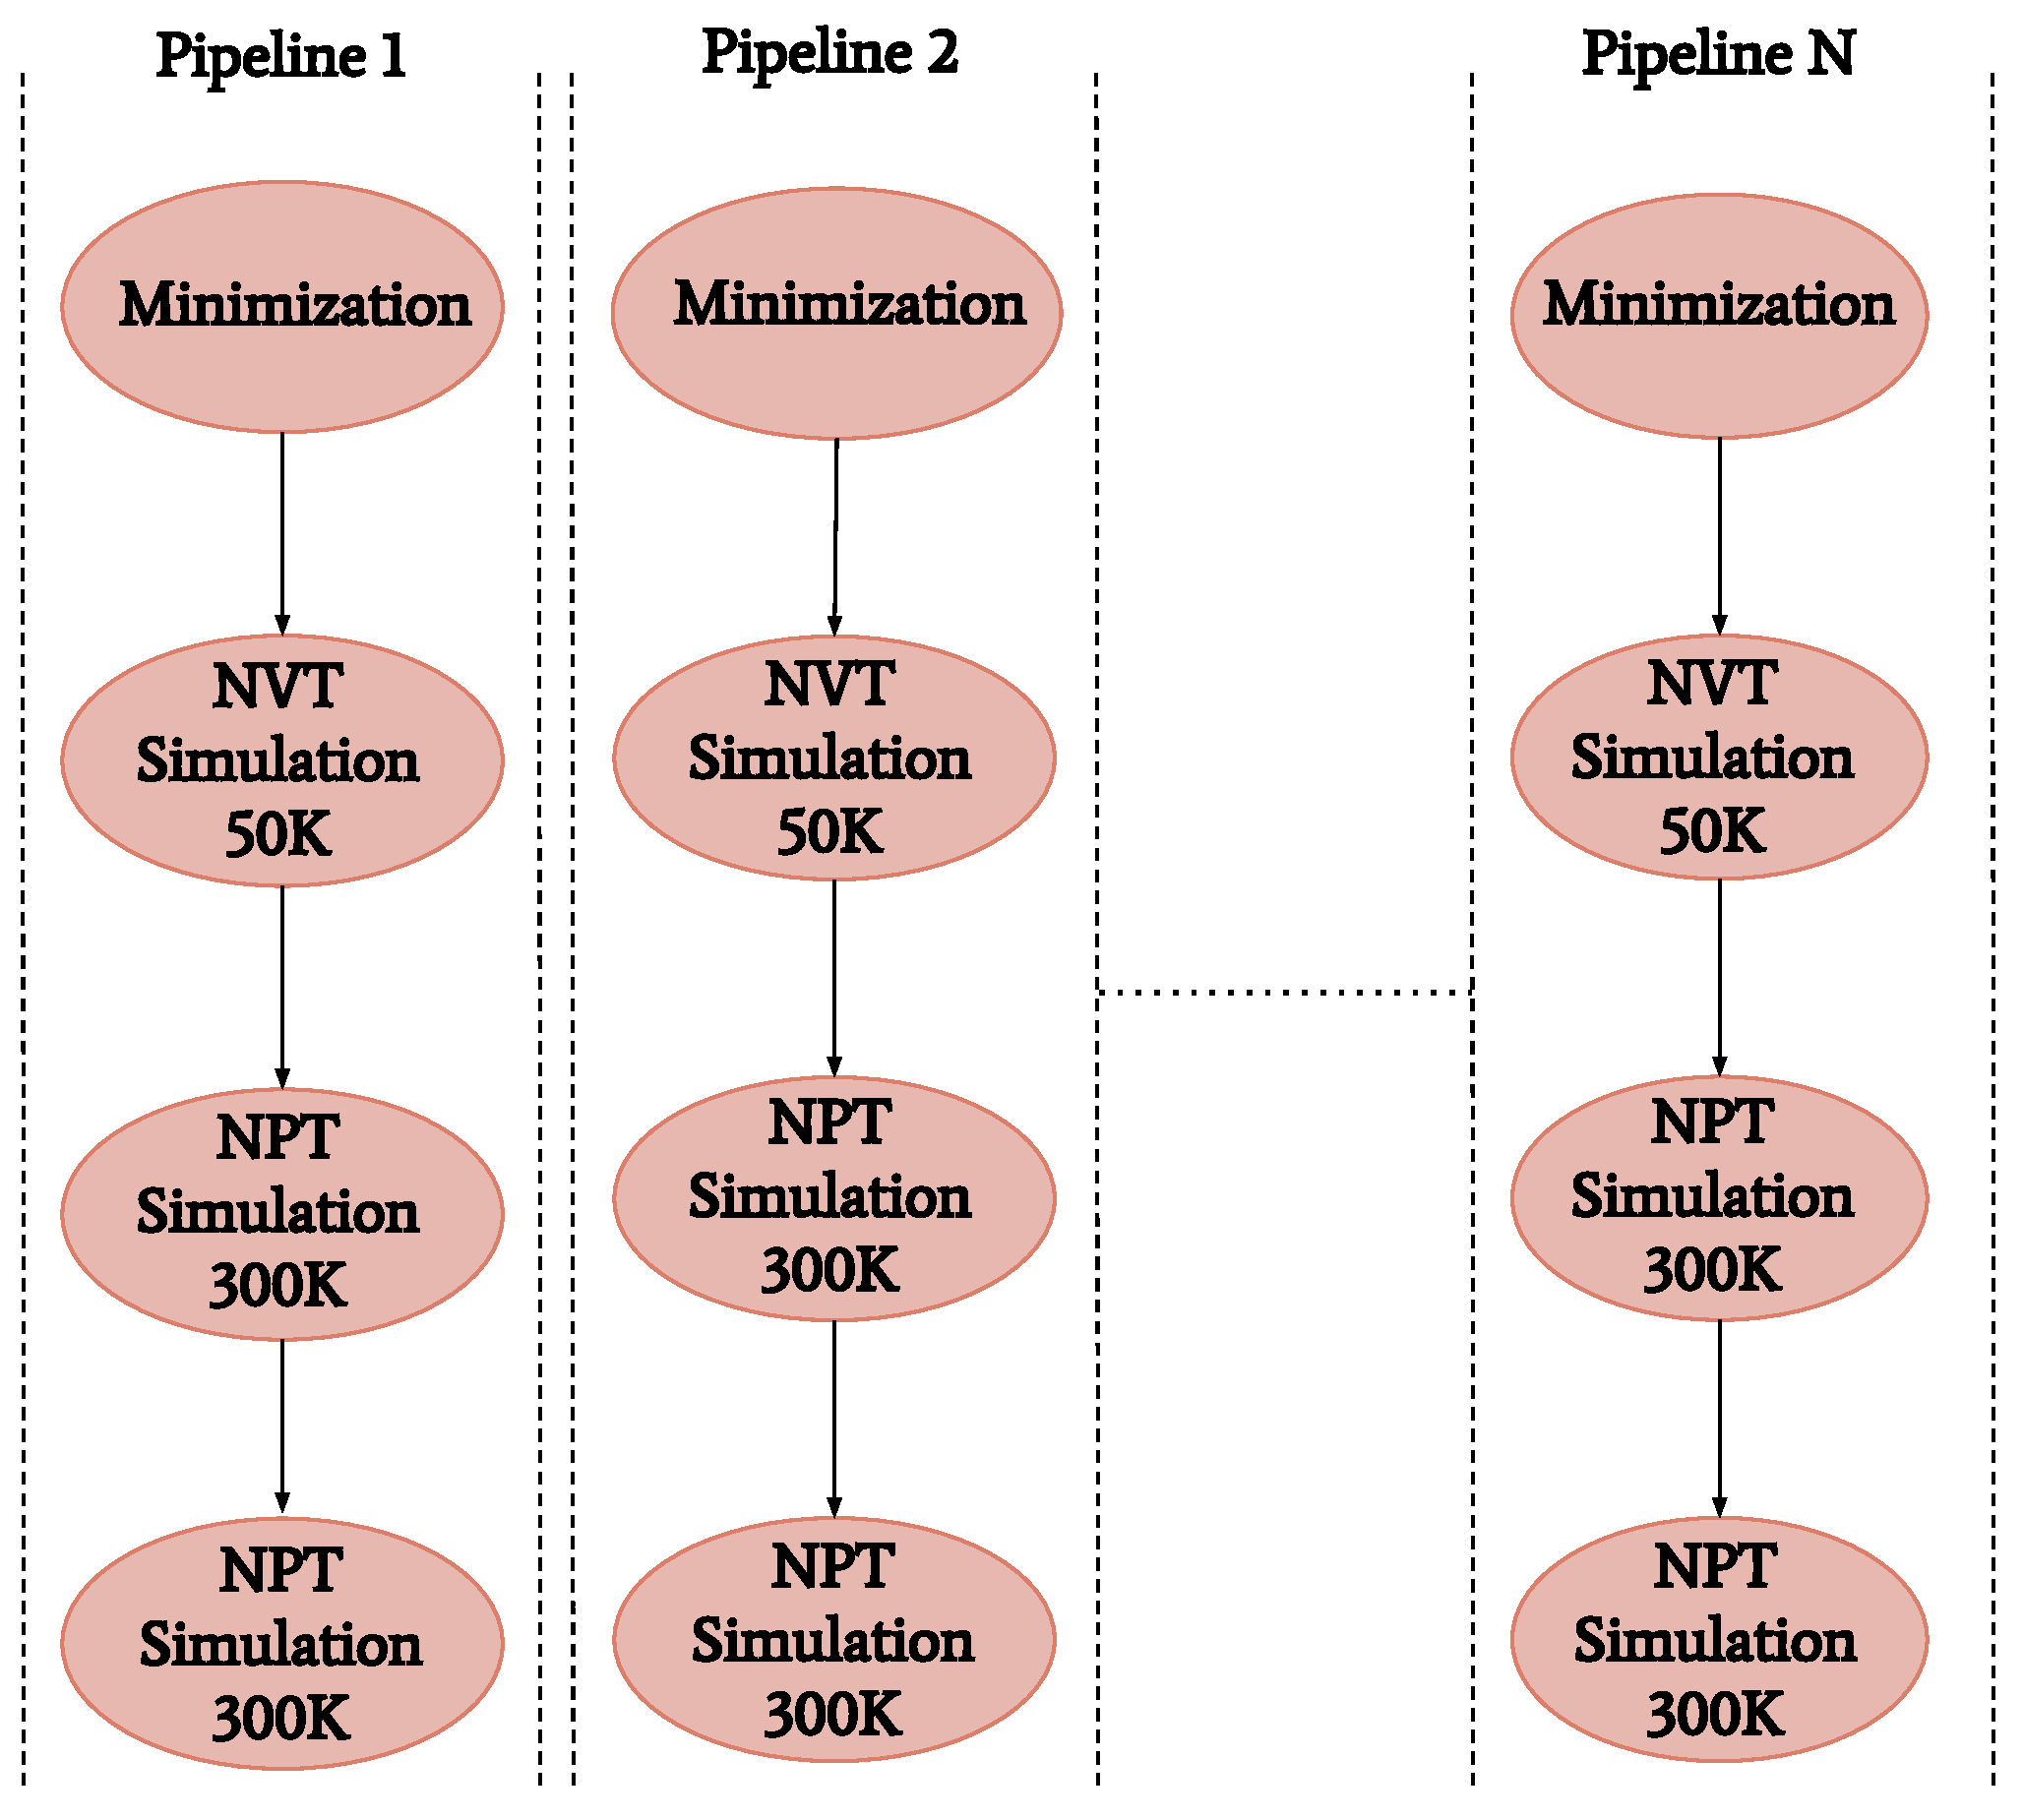
\includegraphics[width=0.4\textwidth]{FIGURES/HT-BAC-NAMD-pipelines-control-flow-only.pdf}
  \caption{\bf ESMACS protocol indicating n-pipelines where each pipeline represents a replica that follows an identical sequence of NAMD tasks.}
   \label{figure:namd-pipelines}
\end{figure}


The ESMACS protocol in HT BAC defines a set of stages where each stage contains a single task. The order of stages and description of each stages is identical for each pipeline:

1) Untar configuration files
2) Preprep 
3) Minimize with decreasing restraints
4) Equilibration: NVT simulation at 50K, with restraints
5) Equilibration: NPT simulation at 300K, with decreasing restraints 
6) Equlibratin: NPT at 300k, no constraints
7) Tar


Each task requires the these base arguments which are defined as follows:

* name of task
* path to executable 
* arguments to executable
* number of cores 

We build each stage by appending from task(s) and generate a pipeline by appending from stage(s). 

Include diagram for pipeline ESMACS protocol (EnTK take a pipeline (new unit) to task translation layer in the EnTK box)

Add code snippets 

How to express ESMACS and how to execute ESMACS

Each stage is a unique task and has a unique argument
Remind the reader of the 7 stages of the ESMACS protocol, and how the stages are expressed, and how the pipelines are added 

